\section{Limits}
\label{sec:limits}
The figure of merit in the examination of possible signal is the di-tau invariant mass ($m_{\tau\tau}$). 
In order to understand if there is an excess in this distribution, the contributions from background sources need to be taken into account.
The background estimates discussed in Section \ref{sec:backgrounds} are compared to the data in the $m_{\tau\tau}$ distribution.
The likelihood of the observed data given the combination of background distributions is taken as binned Poisson likelihood.
The Poisson probability, $p(n|\lambda)$, to observe $n$ events given $\lambda$ expected events is given according to
\begin{equation}
P(n|\lambda) = \frac{\lambda^{n}e^{-\lambda}}{n!}.
\end{equation}
This probability is taken for each bin in the $m_{\tau\tau}$ distribution and the final likelihood is simply the product of $p(n|\lambda)$ in each bin $i$ up to $N_{bin}$,
\begin{equation}
\label{eqn:poissonlikelihood}
\Lagr(n|\lambda) = \prod_{i=1}^{N_{bin}}P(n_{i}|\lambda_{i}) = \prod_{i=1}^{N_{bin}} \frac{\lambda_{i}^{n_{i}}e^{-\lambda_{i}}}{n_{i}!}.
\end{equation}

The uncertainties related with the estimated backgrounds and the shape of the signal samples are taken as nuisance parameters ($\theta$) in the likelihood.
The number of expected events, $\lambda$, is treated as a function of a signal strength parameter $\mu$, and the nuisance parameters.
The expected number of events is broken up into two functions that depend on the nuisance parameters, $s(\theta)$ and $b(\theta)$ representing the expected signal and background yields respectively.
%If we perform a paradigm shift, and treat $\lambda$ as a combination of the signal strength ($\mu$), $s(\theta)$ as the signal expectation, and $b(\theta)$ as the background expectation, 
Equation \ref{eqn:poissonlikelihood} can then be rewritten with the signal strength as the figure of merit,
\begin{equation}
\Lagr(n|\mu, \theta) = \prod_{i=1}^{N_{bin}} \frac{(\mu s_{i} + b_{i})^{n_{i}}e^{-(\mu s_{i}+b_{i})}}{n_{i}!}
\end{equation}
The likelihood can then be considered to be a function of the signal strength parameter ($\mu$) and the nuisance parameters.
The nuisance parameters are modeled as Bayesian priors ($\rho (\theta|\tilde{\theta})$) with the form being dictated by the source of the uncertainty.
Uncertainties that take on positive values are modeled with log-normal distributions, examples of uncertainties with this form are those associated with cross sections, the integrated luminosity, selection efficiencies, etc.
Uncertainties that are statistical in nature, for example arising from a limited number of events in monte carlo simulation, or from the number of events in a control region are modeled as gamma distributions with the width being driven by the number of events in the region.

A test statistic is defined as the profile likelihood ratio which will allow the extraction of only $\mu$ considering that the value of the nuisance parameters are not of interest.
The test statistic used is given as the log of the ratio of two likelihoods,
\begin{equation}
\label{eqn:teststatistic}
q = -2 ln\frac{\Lagr(n|\mu,\hat{\theta}_{\mu})}{\Lagr(n|\hat{\mu},\hat{\theta})},
\end{equation}
where the likelihoods used are maximized while keeping only $\mu$ fixed in the numerator, and both $\mu$ and $\theta$ are allowed to float in the denominator.
The values, $\hat{\mu}$ and $\hat{\theta}$ are then defined as the values at which $\Lagr$ reaches a global maximum.
Two additional constraints are applied to Equation \ref{eqn:teststatistic} such that $\mu$ can not be negative as this would be physically nonsensical, and that $\mu$ must be less than $\hat{\mu}$ enforcing that the limit will represent the upper bound.
The method used to report limits is the modified frequentist construction ($CL_{s}$). 
For the use of this method the systematic uncertainties must be translated from Bayesian priors to probability distribution functions (\emph{pdf}s) via Bayes' theorem,
\begin{equation}
\rho(\theta|\tilde{\theta}) \sim p(\theta|\tilde{\theta})\pi_{\theta}(\theta).
\end{equation}
Here $\pi_{\theta}(\theta)$ are hyper-priors that are chosen to be flat distributions.
The nuisance parameters have the effect of modifying the likelihood in the following way
\begin{equation}
\Lagr(n|\mu, \theta) = \prod_{i=1}^{N_{bin}} \frac{(\mu s_{i} + b_{i})^{n_{i}}e^{-(\mu s_{i}+b_{i})}}{n_{i}!} p(\tilde{\theta}|\theta).
\end{equation}
In the $CL_{s}$ method, values for $\mu$ are obtained by maximizing $\Lagr$ for the signal plus background ($\hat{\theta}_{\mu}^{obs}$) and background only ($\hat{\theta}_{0}^{obs}$) hypotheses.
Two $p$-values are found corresponding to the scenario in which the value of the test statistic ($q_{\mu}$) is greater than the observed value for the test statistic ($q_{\mu}^{obs}$) in the signal plus background ($s+b$) and background only ($b$) hypotheses,
%\begin{equation}
\begin{eqnarray*}
p_{s+b} & = & P\left(q_{\mu} > q_{\mu}^{obs}|\mu(\hat{\theta}_{\mu}^{obs}) + b(\hat{\theta}_{\mu}^{obs})\right), \\
p_{b}   & = & P\left(q_{\mu} > q_{\mu}^{obs}|b(\hat{\theta}_{0}^{obs})\right).
\end{eqnarray*}
%\end{equation}
The $CL_{s}$ is then defined as the ratio of the two $p$-values,
\begin{equation}
CL_{s} = \frac{p_{s+b}}{p_{b}},
\end{equation}
and can be interpreted as the probability that the $q_{\mu}$ is greater than $q_{\mu}^{obs}$, and as such if $CL_{s} = \alpha$ the signal can be excluded at the ($1-\alpha$) confidence level.
The Higgs, given a particular mass and cross section,  can be excluded at the 95\% confidence level by repeating the afore mentioned procedure and adjusting $\mu$ until $CL_{s}$ obtains the value $CL_{s} = 0.05$.

The above procedure is repeated with toy monte carlo pseudo-data in which $\hat{\theta}_{\mu}$ and $\hat{\theta}_{0}$ are taken from the data-driven observed values and the remaining nuisance parameters $\tilde{\theta}$ are randomized according to the modeled $pdf$s.
With a sufficient number of toy monte carlo pseudo-experiments one can obtain the expected limit given the background only hypothesis, as well as $\pm\sigma$ and $\pm 2\sigma$ error bands.
%It should be noted, however that although $\hat{\theta}_{\mu}$ and $\hat{\theta}_{0}$ are taken from the observed values, they are allowed to float in fits needed to evaluate the test statistic. % FIXME THIS SUCKS

Generating a sufficient sample size of pseudo-data leads to a scenario which is very CPU intensive.
It has been shown that in generating the pseudo-data the resulting expectation is only weakly coupled to the nuisance parameters and indeed in the case that $\pi(\theta)$ represents a flat distribution the expected limit can be well approximated without the use of pseudo-data\cite{ASYMPTOTIC}.
In the case where there is only a single parameter of interest the distribution for $\hat{\mu}$ follows a Gaussian distribution,
\begin{equation}
- 2ln\lambda(\mu) = \frac{\mu - \hat{\mu}}{\sigma^{2}} + \mathcal{O}(\frac{1}{\sqrt{N}}).
\end{equation}
Thus the test statistic becomes:
%\begin{equation}
\begin{eqnarray*}
q & = & -2ln\lambda_{\mu} + 2ln\lambda_{0} \\
  & = & \frac{1 - 2\hat{\mu}}{\sigma^{2}},
\end{eqnarray*}
%\end{equation}
and the $p$-values follow.
For the purposes of this analysis, the limits presented will be shown according to this approximation.

In the search for both the SM and MSSM Higgs boson(s), it has been found that increased sensitivity can be obtained by breaking up the search into separate categories that represent the different production mechanisms.
The motivation is that the signal to background ratio will increase in certain categories as seen in Section \ref{sec:categories}.
It is however, desirable to combine the results of each category to obtain a single result.
The nuisance parameters that are common across the separate categories are arranged to be 100\% correlated, either positively or negatively. 
Additionally the categories are mutually exclusive.
This method of producing the categories and the associated nuisance parameters ensures that the categories are statistically independent and the combined likelihood is then a product of the individual likelihoods, and the test statistic is:
\begin{equation}
q = -2ln\frac{\prod_{i}\Lagr_{i}(\mu, \hat{\theta}_{i_{\mu}})}{\prod_{i}\Lagr_{i}(\hat{\mu}, \hat{\theta}_{i})}.
\end{equation}

The improvement in the expected limits assuming no signal can be seen in Figure \ref{fig:expectedlimits}.
Figure \ref{fig:smlimits} shows the observed $95\%$ confidence level limit on the ratio $\frac{\sigma\times BR(H\rightarrow\tau\tau)}{\sigma\times BR(H\rightarrow\tau\tau)_{SM}}$ for the combined standard model categories, and the absolute limit on $\sigma\times BR(H\rightarrow\tau\tau)$ for the combined MSSM categories can be seen in Figure \ref{fig:mssmlimits}.
The observed limits are shown superimposed on the median expected $95\%$ confidence level assuming a null signal with the green bands representing the $\pm\sigma$ error bands, and the yellow bands representing the $\pm 2\sigma$ error bands.
In the standard model one would say that the Higgs has been excluded with a given mass for the portion of the figure where the observed value is less than one. 
In this case the observed limit is found to be approximately three times that predicted by the standard model.
A limit on the absolute cross section in the case of the MSSM search is shown so that the limit on the cross section can be produced independent of $tan\beta$. 
It is found that $\sigma\times BR(H\rightarrow\tau\tau) < 20$ pb for low $m_{A^{0}}$, and $\sigma\times BR(H\rightarrow\tau\tau) < 0.2$ pb for high $m_{A^{0}}$.

\begin{figure}[ht]
\centering
\centerline{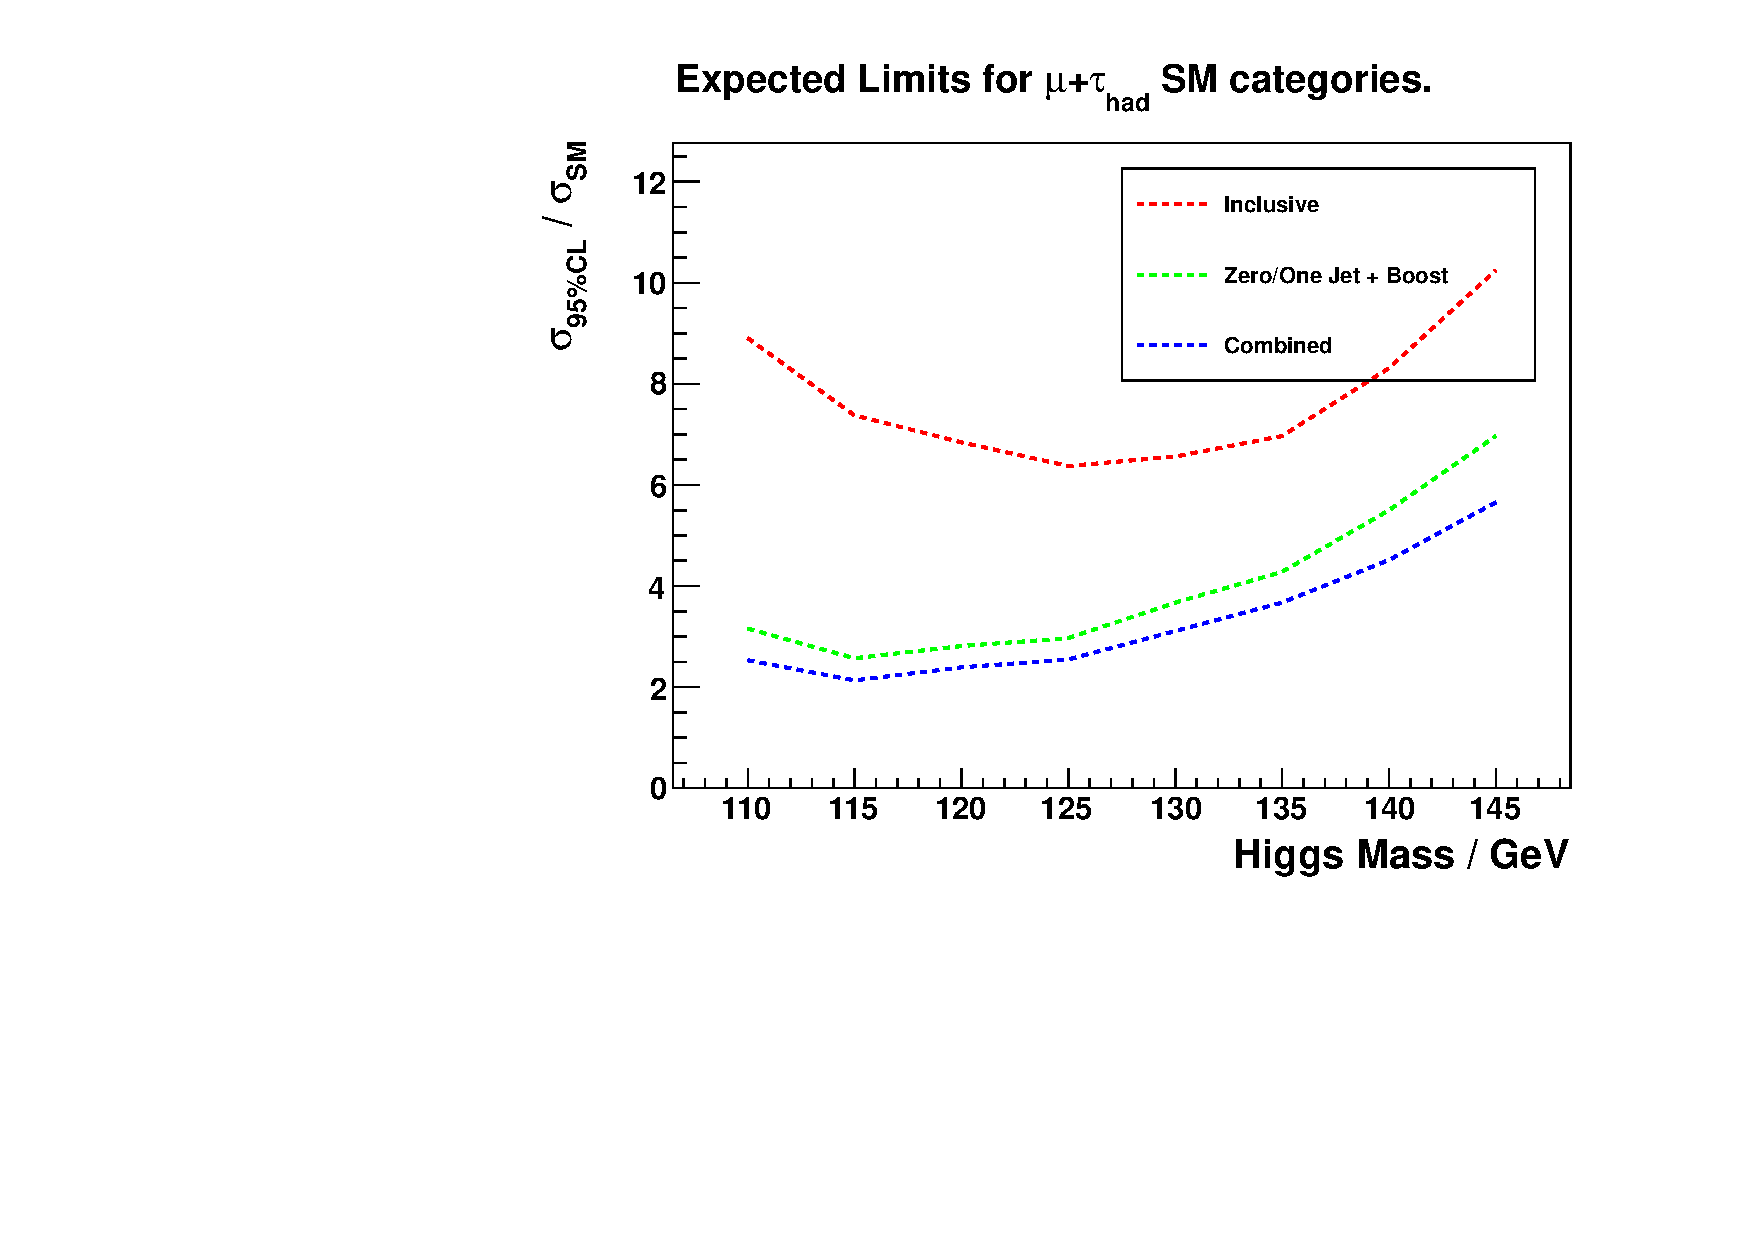
\includegraphics[width=0.45\textwidth]{plots/limitsAHtoMuTau_expected_sm.pdf}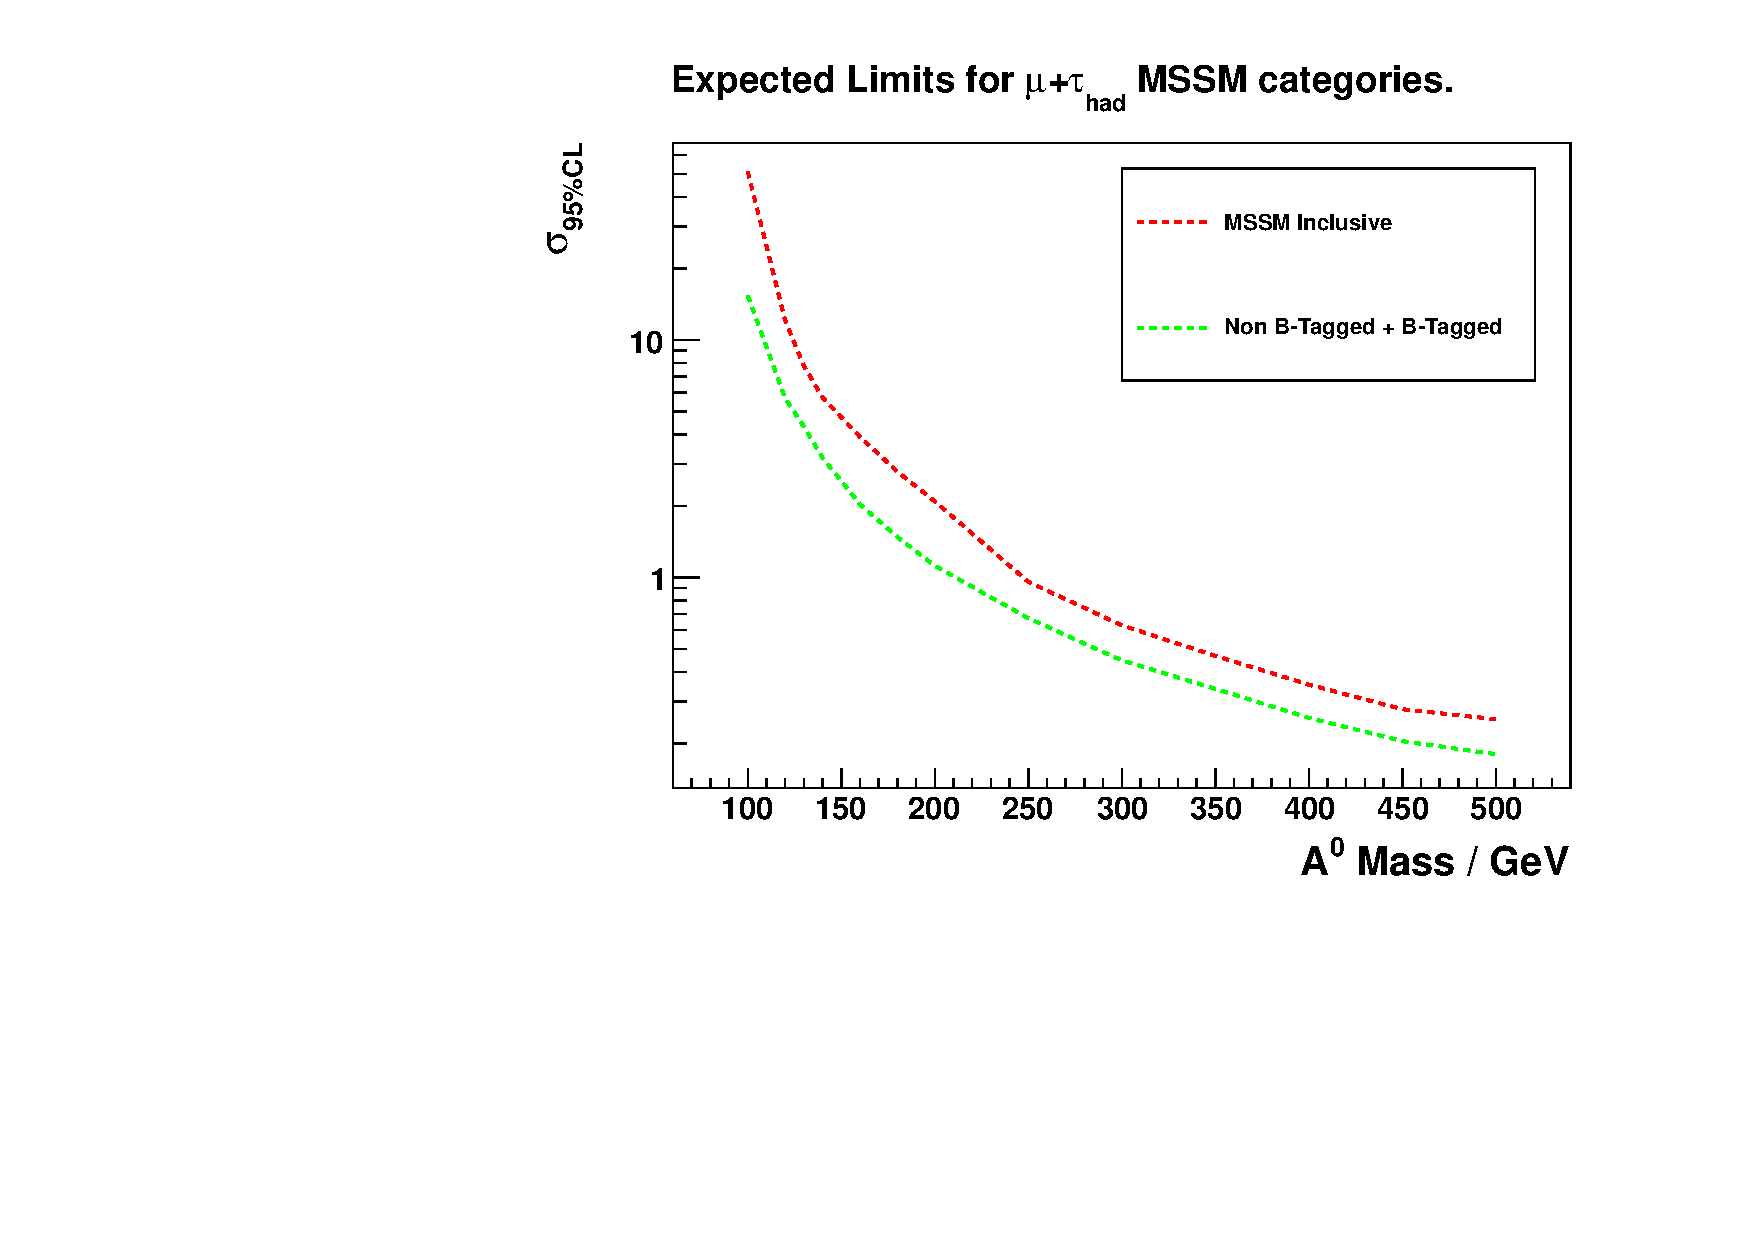
\includegraphics[width=0.45\textwidth]{plots/limitsAHtoMuTau_expected_mssm.pdf}}
\caption{
  Median expected limits for pseudo-data evaluation of the test statistics shown for the inclusive and combined categories of the SM (left) and MSSM (right). 
  The SM limits are reported as the ratio of the measured $\sigma\times BR(H\rightarrow\tau\tau)$  to that predicted by the SM.
  The MSSM limits are reported as the limit on the absolute $\sigma\times BR(H\rightarrow\tau\tau)$.
}
\label{fig:expectedlimits}
\end{figure}

\begin{figure}[ht]
\centering
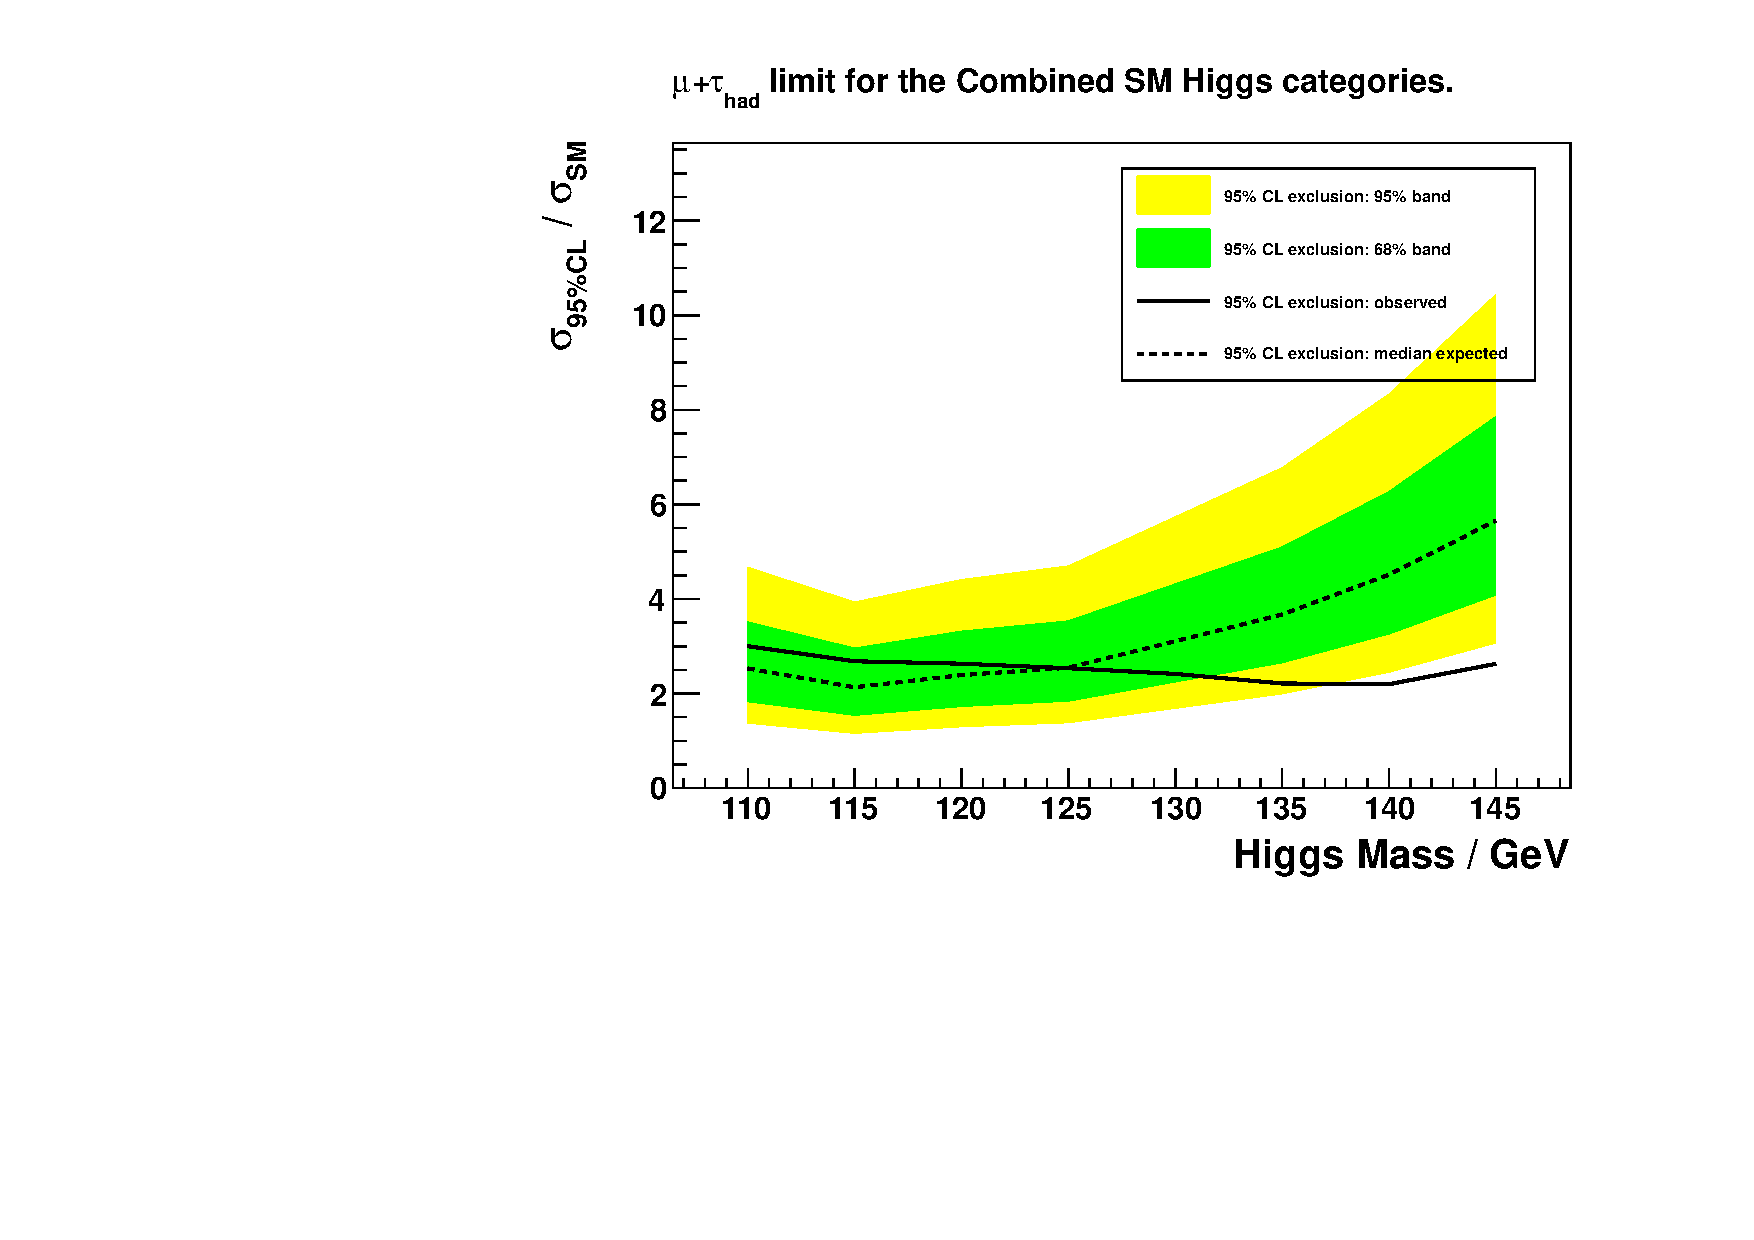
\includegraphics[width=0.95\textwidth]{plots/limitsAHtoMuTau_svFit_sm.pdf}
\caption{Observed ratio $\sigma\times BR(H\rightarrow\tau\tau)/\sigma_{SM}\times BR(H\rightarrow\tau\tau)$ exclusion at $95\%$ confidence level for the combined SM categories compared to the expected and $\pm\sigma$ and $\pm 2\sigma$ error bands.}
\label{fig:smlimits}
\end{figure}

\begin{figure}[ht]
\centering
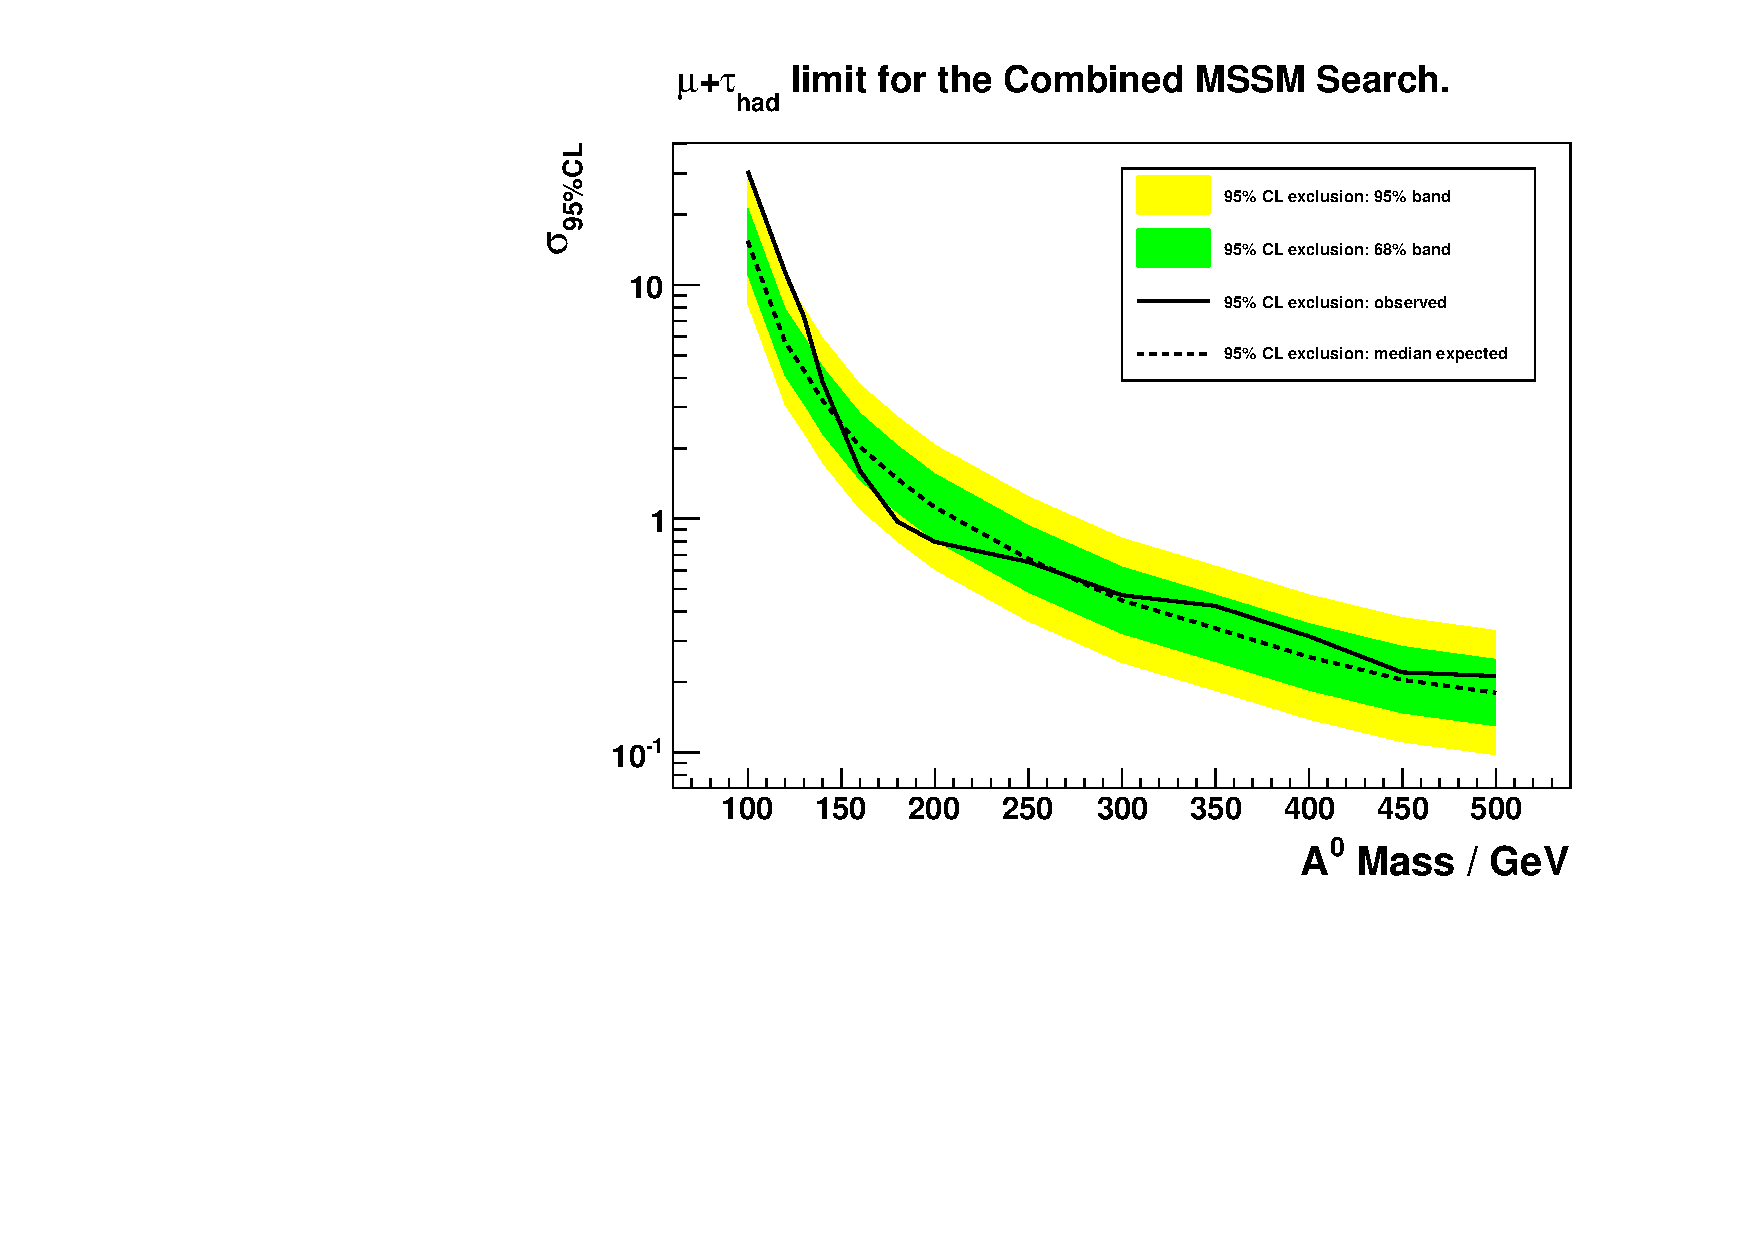
\includegraphics[width=0.95\textwidth]{plots/limitsAHtoMuTau_svFit_mssm.pdf}
\caption{Observed $\sigma\times BR(H\rightarrow\tau\tau)$ exclusion at $95\%$ confidence level for the combined MSSM categories compared to the expected, $\pm\sigma$ and $\pm 2\sigma$ error bands.}
\label{fig:mssmlimits}
\end{figure}

The CP-odd neutral Higgs boson ($A^{0}$) will be mass degenerate with $h_{0}$ at masses lower than $\approx 130$ GeV, and for higher masses $A^{0}$ will be degenerate with $H_{0}$.
The NNLO cross sections and branching ratios to tau leptons for the three neutral Higgs bosons were computed for the range $100 < m_{A^{0}} < 500$ GeV, and $0 < \tan\beta < 50$.
The calculated cross sections and branching ratios are compared to the observed and expected upper limits on the MSSM Higgs boson as seen in Figure \ref{fig:mssmlimits} to produce an exclusion in the $m_{A}$-$\tan\beta$ MSSM plane.
The theoretical uncertainties on the branching ratios, pdfs, and relative contributions of $gg\rightarrow H$ and $gg\rightarrow bbH$ are taken into account by varying the observed exclusion by $\pm1\sigma$.
The exclusion is presented with the previous result of the Tevatron overlaid for reference in Figure \ref{fig:tanbeta}.

\begin{figure}[tpb]
\centering
\centerline{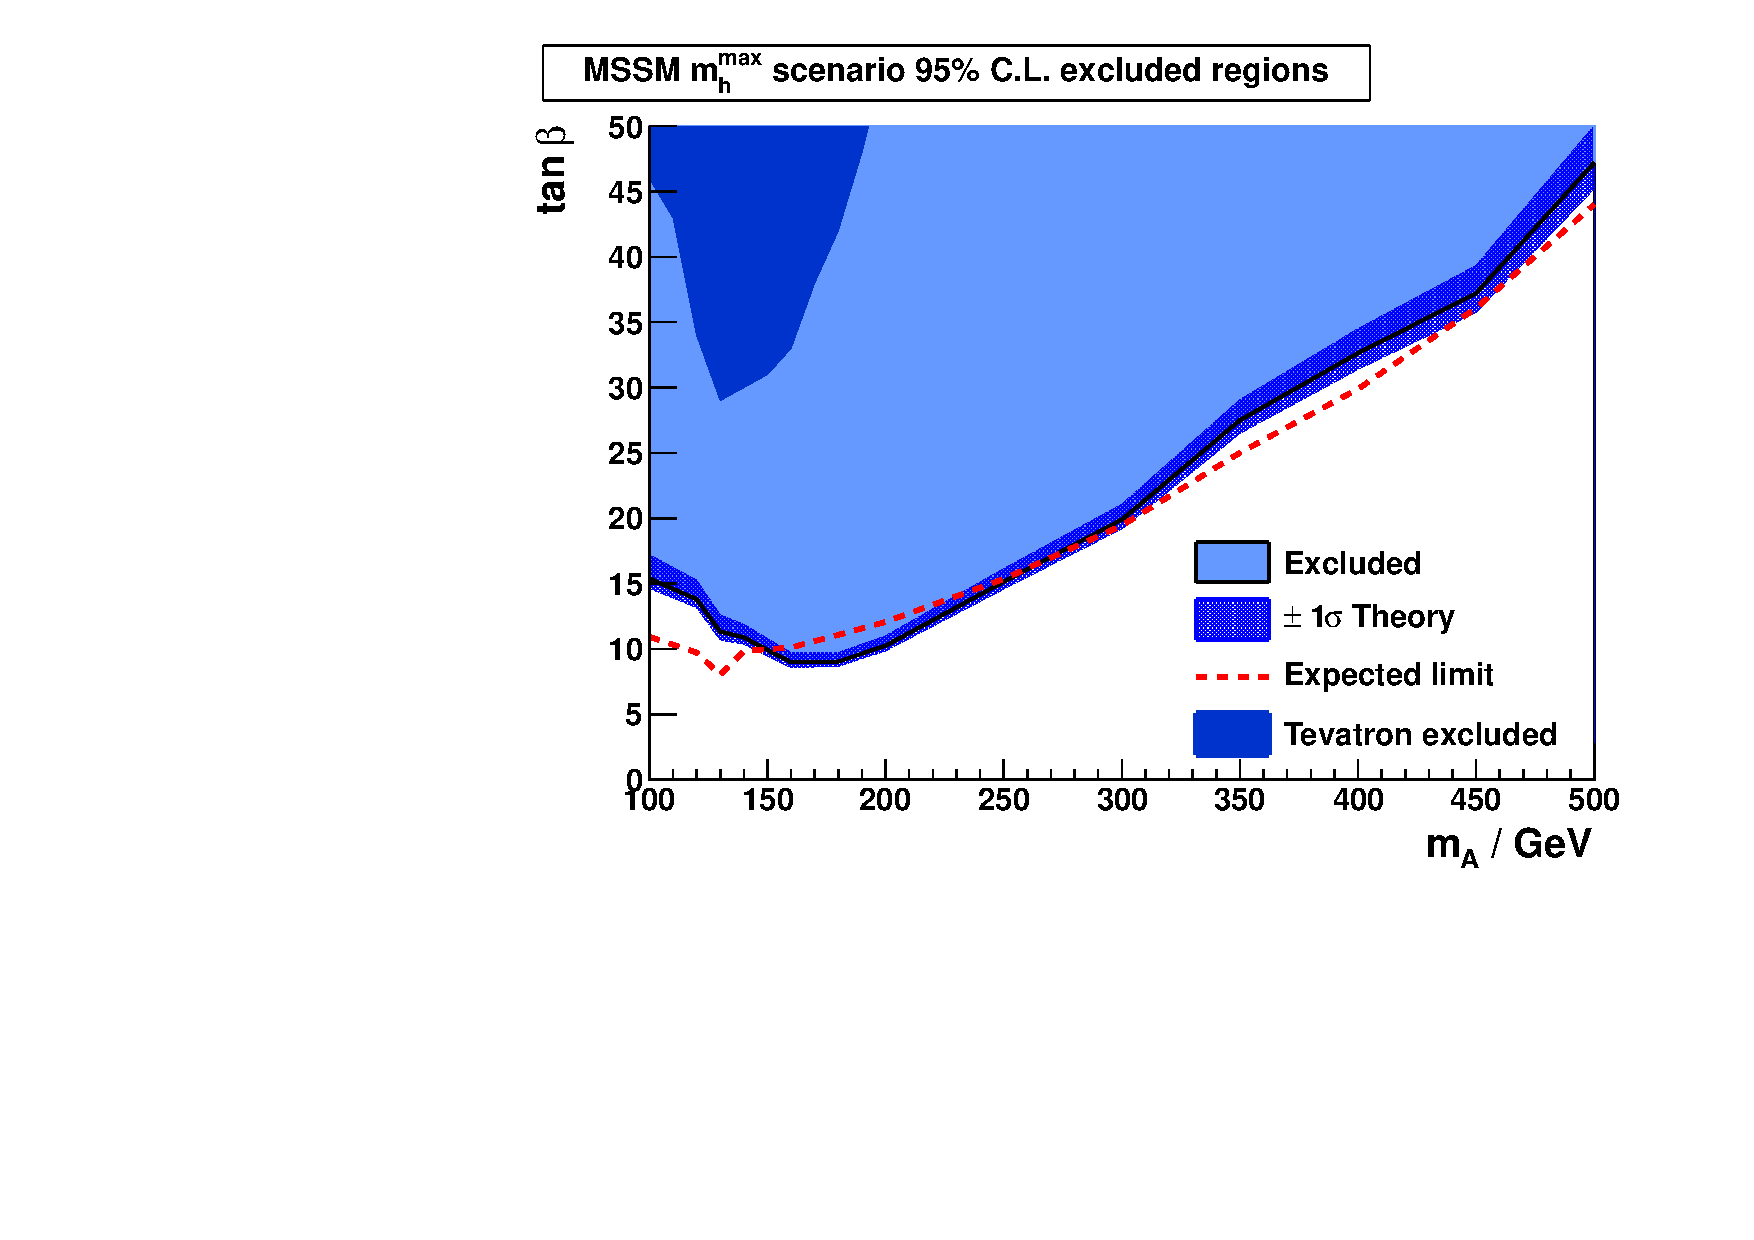
\includegraphics[width=0.95\textwidth]{plots/tan_beta.pdf}}
\caption{
  MSSM exclusion in the $m_{A}$-$tan\beta$ plane extrapolated from the measured upper limit MSSM Higgs cross section.
}
\label{fig:tanbeta}
\end{figure}

